\documentclass[tikz,border=2mm,12pt]{standalone}

\begin{document}
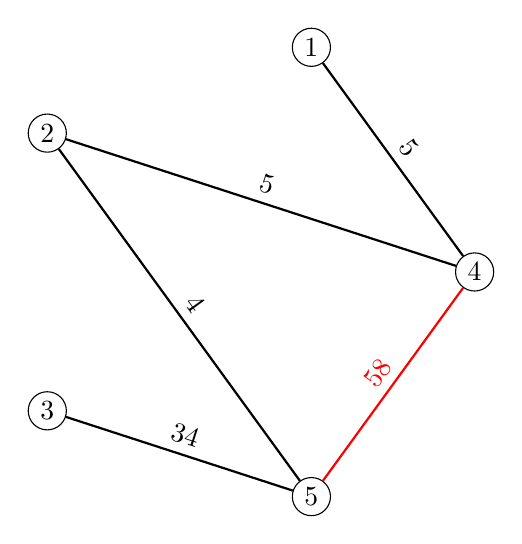
\begin{tikzpicture}[scale=1.5]
    % Define nodes with labels
    \foreach \i/\label in {1/1, 2/2, 3/3, 4/5, 5/4}
    \node[circle, draw, inner sep=2pt] (node\i) at (\i*72:2cm) {\label};

    % Define edges with weights and colors
    \foreach \source/\dest/\weight/\edgecolor in {1/5/5/black, 2/5/5/black, 2/4/4/black, 3/4/34/black, 5/4/58/red}
    \draw[thick, \edgecolor] (node\source) -- node[midway, above, sloped] {\weight} (node\dest);
\end{tikzpicture}
\end{document}
